\subsection{Les chambres à muons}\label{chapter-LHC-section-CMS-subsec-muons}
\begin{wrapfigure}{R}{7.5cm}
\centering
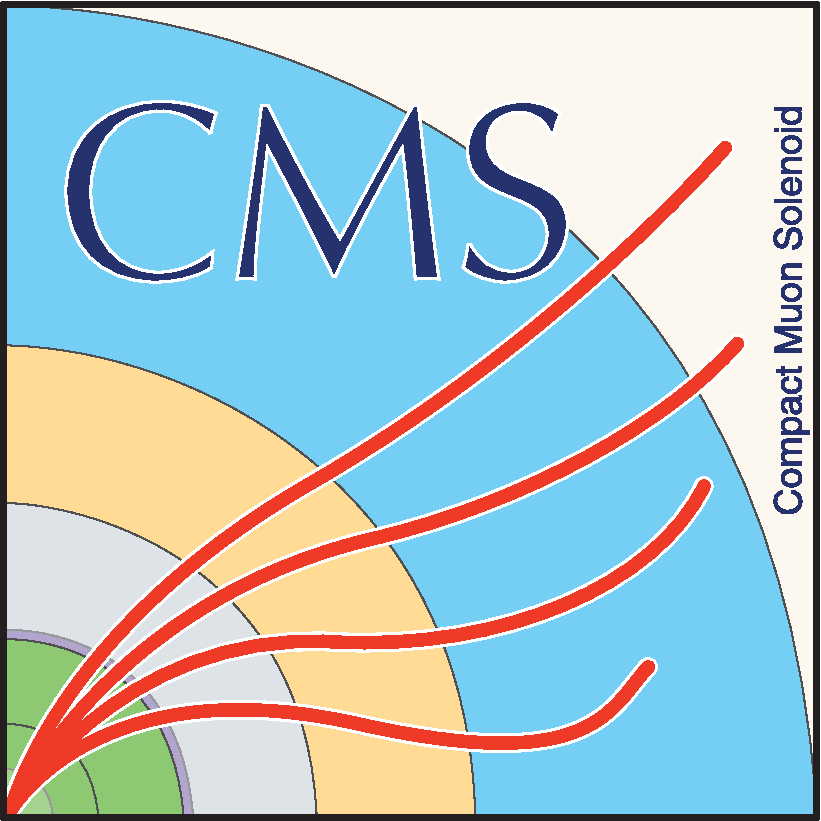
\includegraphics[width=5cm]{\PhDthesisdir/plots_and_images/logos/CMS_logo.pdf}
\caption[Le logo de la collaboration CMS.]{Le logo de la collaboration CMS. Il représente, plié en quatre, un événement $\Higgs\to4\mu$ dans le plan transverse du détecteur.}
\label{fig-CMS_logo}
\end{wrapfigure}
La détection des muons est un enjeu important afin de discriminer les signatures de processus physiques d'intérêt du bruit de fond au LHC~\cite{cms_paper}.
Par exemple, la découverte du boson de Higgs avec le \og canal d'or \fg{} où ce boson de désintègre en deux bosons \Zboson, eux-même se désintégrant en muons, donne une signature à quatre muons.
C'est d'ailleurs ce type d'événement qui a inspiré le logo de la collaboration, figure~\ref{fig-CMS_logo}.
Au-delà de la détection relativement aisée des muons, ils permettent d'obtenir une bien meilleure résolution sur la masse du Higgs qu'avec d'autres particules finales.
Bien d'autres processus physiques impliquent des muons.
Une mesure la plus précise possible des muons ainsi qu'une large couverture angulaire pour leur détection se trouve donc au cœur de la conception du détecteur CMS, comme l'indique le \og M \fg{} de l'acronyme.
%\begin{figure}[h]
%\centering
%\begin{tikzpicture}
%
%{\node[anchor= east,inner sep=0] at (0,0) {\includegraphics[width=.33\textwidth]{\PhDthesisdir/plots_and_images/Event_displays/H_to_4mu_CMS_logo.tex}};}
%
%\draw [thick, -latex] (.25,0) --+ (.75,0);
%\draw (.25,0) + (1,0) coordinate (a);
%
%{\node[anchor=south west,inner sep=0] at (a) {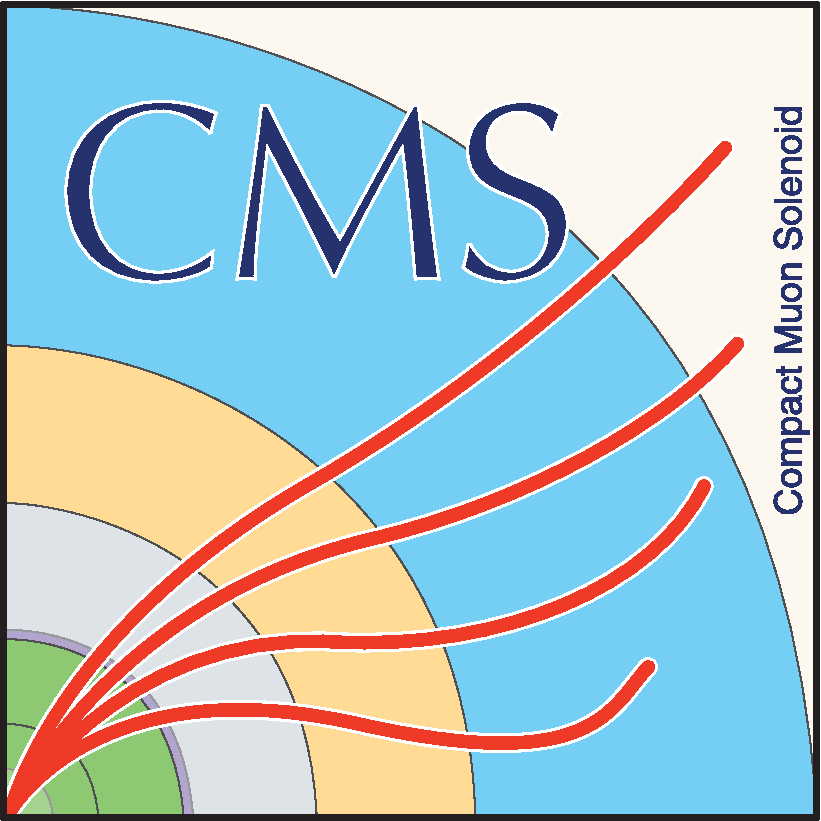
\includegraphics[width=.165\textwidth]{\PhDthesisdir/plots_and_images/logos/CMS_logo.pdf}};}
%
%\draw (-.33\textwidth,0) + (-.25,0) coordinate (b);
%\draw [thick, latex-] (b) --+ (-.75,0);
%\draw (b) + (-1,0) coordinate (c);
%
%{\node[anchor= east,inner sep=0] at (c) {\includegraphics[width=.33\textwidth]{\PhDthesisdir/plots_and_images/Event_displays/H_to_4mu.tex}};}
%\end{tikzpicture}
%\caption[Le logo de la collaboration CMS.]{Le logo de la collaboration CMS. Il représente, plié en quatre, un événement $\Higgs\to\Zboson\Zboson\to4\mu$ dans le plan transverse du détecteur.}
%\label{fig-CMS_logo}
%\end{figure}
\par Les chambres à muons~\cite{cms_paper,CERN-LHCC-97-032,CMS-MUO-11-001,CMS-MUO-16-001}, destinées à la mesure de ces particules, sont encastrées dans la culasse de retour du champ magnétique, \ie\ dans la partie la plus externe du détecteur.
La culasse de retour, décrite dans la section~\ref{chapter-LHC-section-CMS-subsec-solenoide}, permet d'obtenir à l'aide du solénoïde un champ magnétique de \num{1} à \SI{2}{\tesla} dans cette zone~\cite{CMS_magnetic_field}, donnant une bonne résolution sur l'impulsion des muons.
Les autres types de particules ayant été absorbées dans les couches précédentes, seuls les muons atteignent cette partie du détecteur.
La figure~\ref{fig-chapter-LHC-section-CMS-subsec-muons-CMS-MUO-16-001-Figure_001} schématise la structure des chambres à muons dans un cadrant du détecteur.
De par la forme du solénoïde, cette partie du détecteur se divise également en un barillet et deux bouchons.
\begin{figure}[h]
\centering
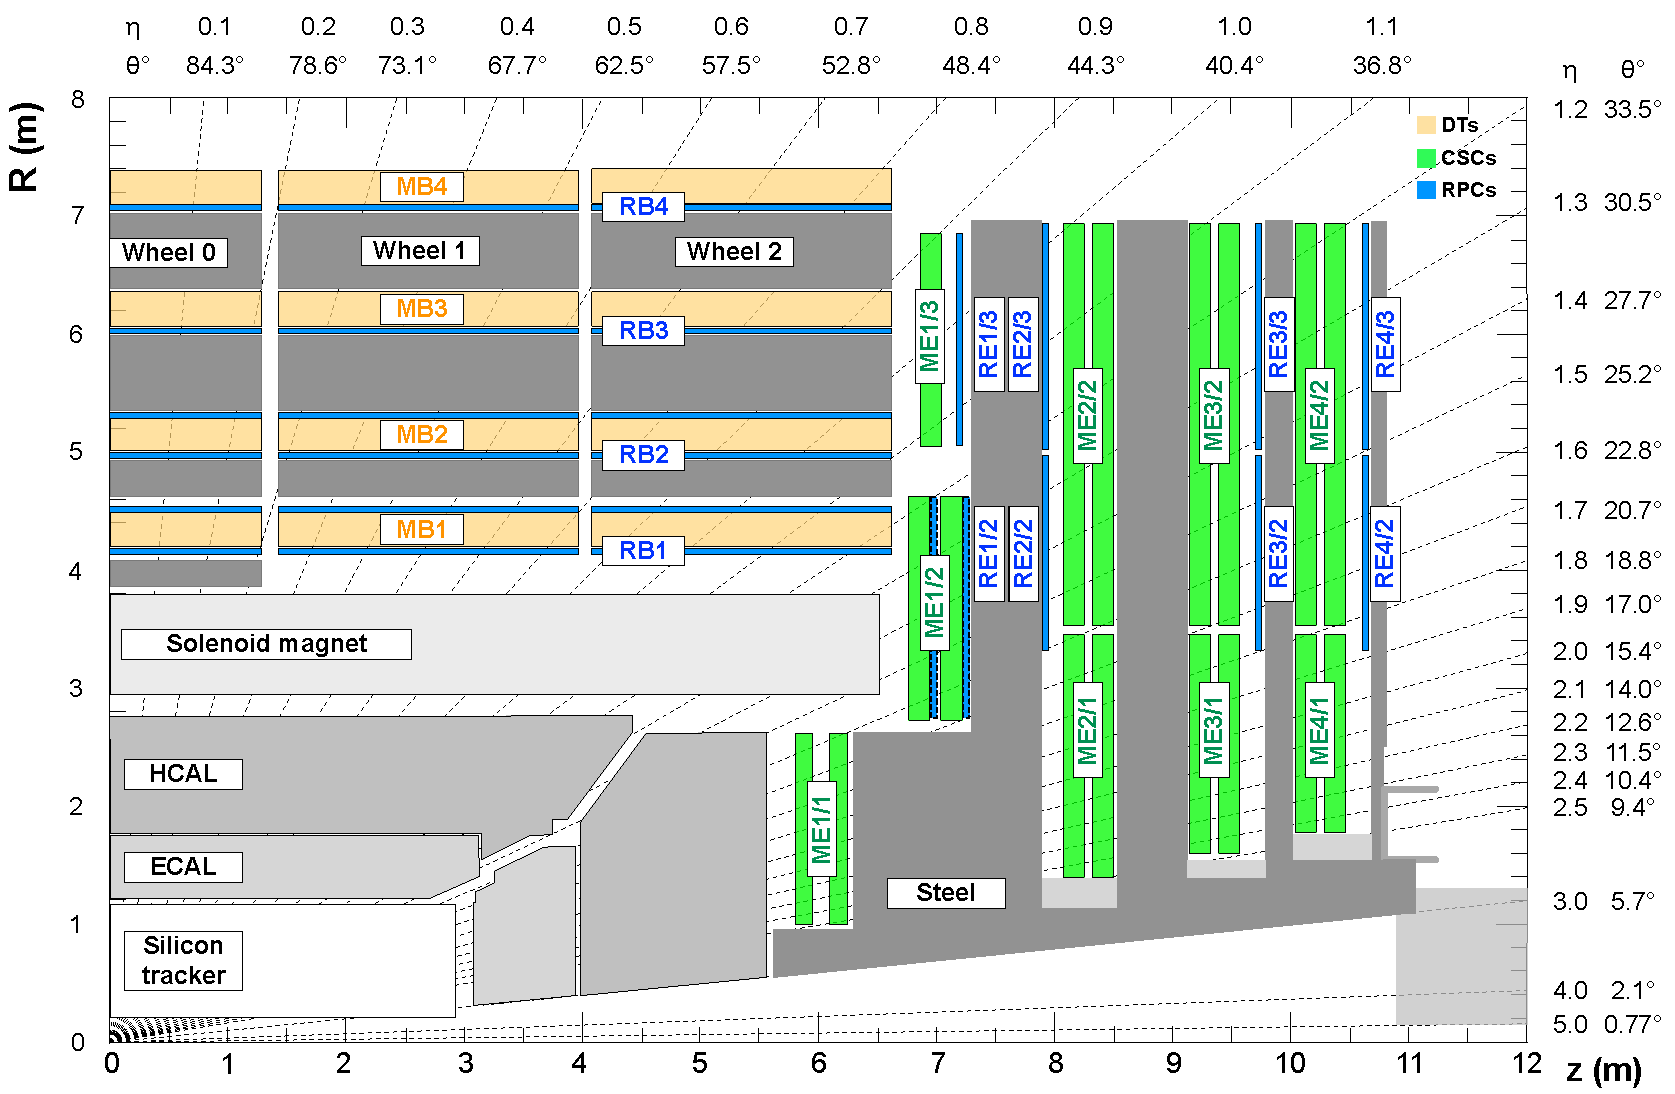
\includegraphics[width=0.8\textwidth]{\PhDthesisdir/plots_and_images/from_CMS-MUO-16-001/Figure_001.pdf}
\caption[Schéma des chambres à muons de CMS.]{Schéma d'un cadrant du détecteur CMS~\cite{CMS-MUO-16-001} montrant la localisation des chambres à muons et leur nature: tubes à dérive (DT, en jaune), chambres à pistes cathodiques (CSC, en vert) et chambres à plaques résistives (RPC, en bleu). Certaines valeurs de $\eta$ et les directions associées sont indiquées.}
\label{fig-chapter-LHC-section-CMS-subsec-muons-CMS-MUO-16-001-Figure_001}
\end{figure}
\par Dans le barillet (MB), cinq roues le long de l'axe du faisceau (numérotées de \num{-2} à \num{2}) couvrent la région $\abs{\eta}<\num{1.2}$.
Une roue est composée de douze segments réalisant un tour complet en $\phi$.
Chaque segment comporte quatre stations ou couches successives de chambres à muons.
Les conditions expérimentales permettent d'y utiliser des chambres à tubes à dérive (DT, \emph{Drift Tubes}).
Les trois premières stations contiennent douze chambres à muons.
Deux groupes de quatre chambres mesurent la position du muon dans le plan transverse et sont séparées autant que possible afin d'obtenir la meilleure résolution angulaire.
Quatre autres chambres donnent cette mesure le long de l'axe du faisceau.
La quatrième station ne comporte pas de mesure selon cet axe.
\par Les bouchons (MB) sont soumis à une quantité plus importante de muons.
Au lieu de tubes à dérives, la technologie utilisée est celle des chambres à pistes cathodiques (CSC, \emph{Cathode Strip Chambers}).
Les CSC présentent un temps de réponse plus court, une segmentation fine ainsi qu'une bonne résistance aux radiations.
Elles couvrent la région $\num{0.9}<\abs{\eta}<\num{2.4}$.
Quatre stations de CSC successives sont installées dans les bouchons et sont orientées radialement par rapport au faisceau, donnant une mesure de précision dans le plan transverse de la position des muons.
%\par distribution de la résolution
%\begin{figure}[h]
%\centering
%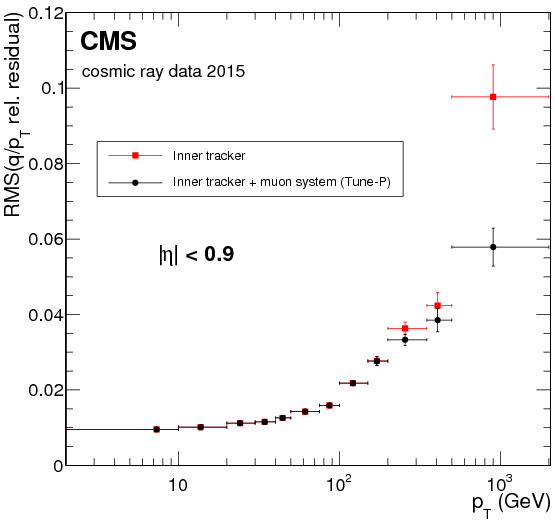
\includegraphics[width=0.8\textwidth]{\PhDthesisdir/plots_and_images/from_CMS-MUO-16-001/Figure_009.png}
%\label{fig-chapter-LHC-section-CMS-subsec-muons-CMS-MUO-16-001-Figure_009}
%\end{figure}
\par Outre l'identification et la mesure des muons, les chambres à muons sont également utilisées afin de déclencher l'enregistrement des données\footnote{Les modalités du rejet ou de l'enregistrement d'un événement sont discutées plus en détails dans la section~\ref{chapter-LHC-section-CMS-subsec-data_taking}.}.
Un système de déclenchement complémentaire aux DT et CSC est ajouté, il s'agit du RB dans le barillet et du RE dans les bouchons.
Il est composé de chambres à plaques résistives (RPC, \emph{Resistive Plate Chambers}) fournissant des signaux indépendants des DT et CSC, rapides (moins de \SI{25}{\nano\second}) et proposant une bascule\footnote{La bascule est la densité de probabilité de donner un signal ou non. Il est en général favorable d'avoir une bascule rapide à une valeur définie afin de limiter le domaine de réponse aléatoire.} en fonction de l'impulsion transverse très rapide.
La figure~\ref{fig-chapter-LHC-section-CMS-subsec-muons-CMS-MUO-16-001-Figure_016} montre la distribution de la masse invariante des systèmes de deux muons sélectionnés par ce système de déclenchement.
Ces résultats montrent la capacité du détecteur CMS à identifier les muons, se déclencher vis-à-vis de leur présence, de reconstruire leurs propriétés cinématiques et d'identifier ainsi sans ambiguïté les particules dont la désintégration donne ces muons sur une large gamme d'énergie~\cite{CMS-MUO-16-001}.
La caractérisation complète des muons, abordée dans la section~\ref{chapter-LHC-section-evt_reco-subsec-ptc_ID}, utilise conjointement les informations du trajectographe et des chambres à muons.
\begin{figure}[h]
\centering
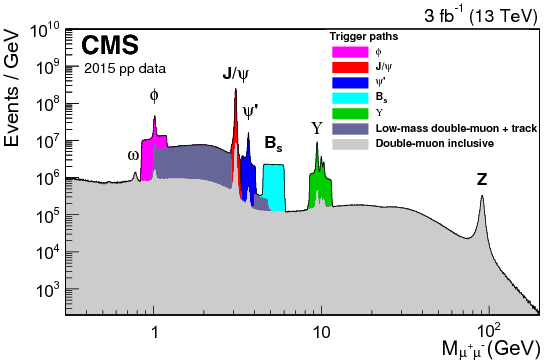
\includegraphics[width=.6\textwidth]{\PhDthesisdir/plots_and_images/from_CMS-MUO-16-001/Figure_016.png}
\caption[Distribution de la masse invariante de deux muons.]{Distribution de la masse invariante du système de deux muons obtenue à partir du système de déclenchement des chambres à muons~\cite{CMS-MUO-16-001}. Les données ont été récoltées en 2015 à l'aide d'un déclenchement global (gris) ainsi que plusieurs déclenchements spécifiques (en couleur). Les résonances de diverses particules apparaissent distinctement.}
\label{fig-chapter-LHC-section-CMS-subsec-muons-CMS-MUO-16-001-Figure_016}
\end{figure}